\section{Sequential Chips}

  So far, the Boolean/arithmetic chips we worked with are \textit{combinational}, which compute functions that depend solely on combinations of their input values.  These provide many processing functions (like the ALU), but that cannot maintain a state. Since computers must be able to not only compute values but also store and recall them, they must be equipped with memory elements that can preserve data over time. These memory elements are built from \textit{sequential chips}. 

  It stores data, which we have developed encoding schemes for, plus \textit{instructions}, which we will talk about next chapter. 

  The act of ``remembering something'' is inherently time-dependent. You remember now what has been committed to memory before. Thus, in order to build chips that remember information, we must first develop some standard means for representing the progression of time. 

  \begin{definition}[Clock] 
    The \textbf{master clock} in a computer is an oscillator that alternates continuously between two phases---labeled $0/1$, low/high,. tick/tock, etc. 
    \begin{enumerate}
      \item The elapsed time between the beginning of $0$ and the end of $1$ is called a \textbf{cycle}, which models one discrete time unit. 
      \item The current \textbf{clock phase} refers to whether it is $0$ or $1$ now. Using the hardware circuitry, the signal is simultaneously broadcast to every sequential chip throughout the computer platform. 
    \end{enumerate}
  \end{definition}

\subsection{Latches and Flip Flops}

  Ideally, we would like a way to store a bit in memory, and this can be done by cross-coupling gates with each other, forming a sort of positive feedback.\footnote{Note that unlike combinational logic, this now deviates from straight-line programming.} Therefore, given a certain signal into our circuit, the outputs remain locked---or ``latched''---into a state. 

  The SR latch---like all electronic circuits---require power to work, labeled with $S$ and $R$. The output is really just $Q$, but we can add redundancy by making the inverse $\overline{Q}$ available as well. 

  \begin{definition}[SR Latch]
    The \textbf{set-reset (SR) latch} is a circuit to store 1-bit memory. This is based on \textit{pulses} and we do not care about the duration of a signal. That is, if we activate a signal to inputs $S, R$ at \textit{any} point in time, then the output $Q$ will remain locked in some state, even \textit{after} the input signal disappears. There are two implementations of an SR latch, which have symmetric behaviors. 

    In XOR latches, 
    \begin{enumerate}
      \item The default state is $R = 0, S = 0$, i.e. they are both \textit{low states}, and $Q$ may be either $0$ or $1$. This is known as an \textbf{active high SR latch}. 
      \item If we send a signal $R = 1$, then $Q = 0$, and even if we reset $R = 0$, $Q$ is still locked at $0$. 
      \item If we send a signal $S = 1$, then $Q = 1$, and even if reset $S = 0$, $Q$ is still locked at $1$. 
      \item Setting both $R = S = 1$ would result in an invalid state since they would attempt to turn $Q$ back and forth between $0$ and $1$, giving us a race condition. 
    \end{enumerate}

    \begin{figure}[H]
      \centering
      \begin{subfigure}[b]{0.48\textwidth}
        \centering
        \begin{tikzpicture}[circuit logic US]
          \node[nor gate] (nor1) at (0, 1) {}; 
          \node[nor gate] (nor2) at (0, -1) {}; 

          \node[left] at (-1.5, 1.1) {$R$}; 
          \node[left] at (-1.5, -1.1) {$S$}; 
          \node[right] at (2, 1) {$Q$};
          \node[right] at (2, -1) {$\overline{Q}$};

          \draw (-1.5, 1.1) -| (nor1.input 1);
          \draw (-1.5, -1.1) -| (nor2.input 2);
          \draw (nor1.output) |- (2, 1); 
          \draw (nor2.output) |- (2, -1); 

          \draw (nor1.output) |- (1.5, 1) -- (1.5, 0.8) -- (-1, -0.7) -- (-1, -0.9) |- (nor2.input 1);
          \draw (nor2.output) |- (1.5, -1) -- (1.5, -0.8) -- (-1, 0.7) -- (-1, 0.9) |- (nor1.input 2);
          \fill (1.5,1) circle (1.5pt);
          \fill (1.5,-1) circle (1.5pt);
        \end{tikzpicture} 
        \caption{Circuit diagram.}
      \end{subfigure}
      \hfill 
      \begin{subfigure}[b]{0.48\textwidth}
        \centering
        \begin{tabular}{|c|c|c|c|}
          \hline
          \textbf{S} & \textbf{R} & \textbf{Q} & \textbf{$\overline{Q}$} \\
          \hline
          0 & 0 & 1 & 0 \\
            &   & 0 & 1 \\
          \hline
          0 & 1 & 0 & 1 \\
          \hline
          1 & 0 & 1 & 0 \\
          \hline
          1 & 1 & 0 & 0 \\
          \hline
        \end{tabular} 
        \caption{Truth table. Note that $S=1, R=1$ is not a valid signal.}
      \end{subfigure}
      \caption{XOR SR Latch. This is }
    \end{figure}

    In XOR latches, this is the opposite
    \begin{enumerate}
      \item The default state is $R = 1, S = 1$, i.e. they are both \textit{high states}, and $Q$ may be either $0$ or $1$. This is known as an \textbf{active low SR latch}.
      \item If we send a signal $R = 0$, then $Q = 1$, and even if we reset $R = 1$, $Q$ is still locked at $1$. 
      \item If we send a signal $S = 0$, then $Q = 0$, and even if reset $S = 1$, $Q$ is still locked at $0$. 
      \item Setting both $R = S = 0$ would result in an invalid state since they would attempt to turn $Q$ back and forth between $0$ and $1$, giving us a race condition. 
    \end{enumerate}

    \begin{figure}[H]
      \centering
      \begin{subfigure}[b]{0.48\textwidth}
        \centering
        \begin{tikzpicture}[circuit logic US]
          \node[nand gate] (nor1) at (0, 1) {}; 
          \node[nand gate] (nor2) at (0, -1) {}; 
          \node[left] at (-1.5, 1.1) {$R$}; 
          \node[left] at (-1.5, -1.1) {$S$}; 
          \node[right] at (2, 1) {$Q$};
          \node[right] at (2, -1) {$\overline{Q}$};

          \draw (-1.5, 1.1) -| (nor1.input 1);
          \draw (-1.5, -1.1) -| (nor2.input 2);
          \draw (nor1.output) |- (2, 1); 
          \draw (nor2.output) |- (2, -1); 

          \draw (nor1.output) |- (1.5, 1) -- (1.5, 0.8) -- (-1, -0.7) -- (-1, -0.9) |- (nor2.input 1);
          \draw (nor2.output) |- (1.5, -1) -- (1.5, -0.8) -- (-1, 0.7) -- (-1, 0.9) |- (nor1.input 2);
          \fill (1.5,1) circle (1.5pt);
          \fill (1.5,-1) circle (1.5pt);
        \end{tikzpicture} 
        \caption{Circuit diagram.}
      \end{subfigure}
      \hfill 
      \begin{subfigure}[b]{0.48\textwidth}
        \centering
        \begin{tabular}{|c|c|c|c|}
          \hline
          \textbf{S} & \textbf{R} & \textbf{Q} & \textbf{$\overline{Q}$} \\
          \hline
          0 & 0 & 1 & 1 \\
          \hline
          0 & 1 & 1 & 0 \\
          \hline
          1 & 0 & 0 & 1 \\
          \hline
          1 & 1 & 0 & 1 \\
            &   & 1 & 0 \\
          \hline
        \end{tabular}
        \caption{Truth table. Note that $S=0, R=0$ is not a valid signal.}
      \end{subfigure}
      \caption{NAND SR Latch}
    \end{figure}
  \end{definition}

  These signals may be noisy, and we might want more control over whether a latch can change states, i.e its \textit{transparency}. This is done by adding an extra \textit{gate} that explicitly tells us when the latch can change states. 

  \begin{definition}[Gated SR Latch]
    A \textbf{gated SR latch} is an SR latch that can only change state when it is enabled. This enabling is done with an additional 2 NAND gates, and so the SR latch is enabled only when $E = 1$. 

    \begin{figure}[H]
      \centering
      \begin{subfigure}[b]{0.48\textwidth}
        \centering
        \begin{tikzpicture}[circuit logic US]
          \node[nand gate] (nand1) at (-2, 1.1) {};
          \node[nand gate] (nand2) at (-2, -1.1) {};
          \node[nor gate] (nor1) at (0, 1) {}; 
          \node[nor gate] (nor2) at (0, -1) {}; 

          \draw (-3, 1.2) -- (nand1.input 1);
          \draw (-3, -1.2) -- (nand2.input 2);
          \draw (-3, 0) -- (-2.7, 0) -- (-2.7,1) -- (nand1.input 2);
          \draw (-3, 0) -- (-2.7, 0) -- (-2.7,-1) -- (nand2.input 1);
          \node[left] at (-3,0) {$E$};
          \node[left] at (-3,1.2) {$R$};
          \node[left] at (-3,-1.2) {$S$};
          \node[right] at (2, 1) {$Q$};
          \node[right] at (2, -1) {$\overline{Q}$};

          \draw (nand1.output) -- (nor1.input 1);
          \draw (nand2.output) -- (nor2.input 2);
          \draw (nor1.output) -- (2, 1); 
          \draw (nor2.output) -- (2, -1); 

          \draw (nor1.output) -- (1.5, 1) -- (1.5, 0.8) -- (-1, -0.7) -- (-1, -0.9) -- (nor2.input 1);
          \draw (nor2.output) -- (1.5, -1) -- (1.5, -0.8) -- (-1, 0.7) -- (-1, 0.9) -- (nor1.input 2);
          \fill (1.5,1) circle (1.5pt);
          \fill (1.5,-1) circle (1.5pt);
          \fill (-2.7,0) circle (1.5pt);
        \end{tikzpicture} 
        \caption{Gated XOR SR Latch.}
      \end{subfigure}
      \hfill 
      \begin{subfigure}[b]{0.48\textwidth}
        \centering
        \begin{tikzpicture}[circuit logic US]
          \node[nand gate] (nand1) at (-2, 1.1) {};
          \node[nand gate] (nand2) at (-2, -1.1) {};
          \node[nand gate] (nor1) at (0, 1) {}; 
          \node[nand gate] (nor2) at (0, -1) {}; 

          \draw (-3, 1.2) -- (nand1.input 1);
          \draw (-3, -1.2) -- (nand2.input 2);
          \draw (-3, 0) -- (-2.7, 0) -- (-2.7,1) -- (nand1.input 2);
          \draw (-3, 0) -- (-2.7, 0) -- (-2.7,-1) -- (nand2.input 1);
          \node[left] at (-3,0) {$E$};
          \node[left] at (-3,1.2) {$R$};
          \node[left] at (-3,-1.2) {$S$};
          \node[right] at (2, 1) {$Q$};
          \node[right] at (2, -1) {$\overline{Q}$};

          \draw (nand1.output) -- (nor1.input 1);
          \draw (nand2.output) -- (nor2.input 2);
          \draw (nor1.output) -- (2, 1); 
          \draw (nor2.output) -- (2, -1); 

          \draw (nor1.output) -- (1.5, 1) -- (1.5, 0.8) -- (-1, -0.7) -- (-1, -0.9) -- (nor2.input 1);
          \draw (nor2.output) -- (1.5, -1) -- (1.5, -0.8) -- (-1, 0.7) -- (-1, 0.9) -- (nor1.input 2);
          \fill (1.5,1) circle (1.5pt);
          \fill (1.5,-1) circle (1.5pt);
          \fill (-2.7,0) circle (1.5pt);
        \end{tikzpicture} 
        \caption{Gated NAND SR Latch.}
      \end{subfigure}
      \caption{}
    \end{figure}
  \end{definition}

  \begin{example}[Gated SR Latch]
    Let's run some simulations. 

    \begin{figure}[H]
      \centering 
      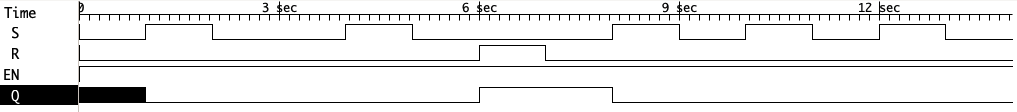
\includegraphics[width=\textwidth]{img/gated_sr1.png}
      \caption{We keep $E=1$ the whole time.} 
    \end{figure}

    \begin{figure}[H]
      \centering 
      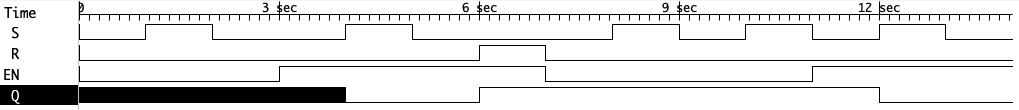
\includegraphics[width=\textwidth]{img/gated_sr2.png}
      \caption{We enable and disable $E$ throughout.} 
    \end{figure}
  \end{example}

  Note that we still have the problem of invalid signals. For example, if there was an instance that at the same clock time a signal of $S=1, R=1$ (on either an ungated latch or a gated latch with $E=1$), then both $Q$ and $\overline{Q}$ will be $1$, which will cause both to be $0$, and then $1$, and so on. This causes a race condition, which leads to unpredictable behavior. 

  \begin{figure}[H]
    \centering 
    \begin{tikzpicture}[circuit logic US]
      \node[nand gate] (nand1) at (-2, 1.1) {};
      \node[nand gate] (nand2) at (-2, -1.1) {};
      \node[nor gate] (nor1) at (0, 1) {}; 
      \node[nor gate] (nor2) at (0, -1) {}; 
      \node[not gate, point down, scale=0.8] (not1) at (-3.5, 0.8) {};

      \draw (-4, 1.2) -- (nand1.input 1);
      \draw (-4, 1.2) -- (-3.5, 1.2) -- (not1.input); 
      \draw (not1.output) -- (-3.5, 0.1) -- (-3.4, 0) -- (-3.5, -0.1) -- (-3.5, -1.2) -- (nand2.input 2);
      \draw (-4, 0) -- (-2.7, 0) -- (-2.7,1) -- (nand1.input 2);
      \draw (-4, 0) -- (-2.7, 0) -- (-2.7,-1) -- (nand2.input 1);
      \node[left] at (-4,0) {$E$};
      \node[left] at (-4,1.2) {$D$};
      \node[right] at (2, 1) {$Q$};
      \node[right] at (2, -1) {$\overline{Q}$};

      \draw (nand1.output) -- (nor1.input 1);
      \draw (nand2.output) -- (nor2.input 2);
      \draw (nor1.output) -- (2, 1); 
      \draw (nor2.output) -- (2, -1); 

      \draw (nor1.output) -- (1.5, 1) -- (1.5, 0.8) -- (-1, -0.7) -- (-1, -0.9) -- (nor2.input 1);
      \draw (nor2.output) -- (1.5, -1) -- (1.5, -0.8) -- (-1, 0.7) -- (-1, 0.9) -- (nor1.input 2);
      \fill (1.5,1) circle (1.5pt);
      \fill (1.5,-1) circle (1.5pt);
      \fill (-2.7,0) circle (1.5pt);
    \end{tikzpicture} 
    \caption{} 
  \end{figure}

  It turns out that we can simplify this circuit a bit more, giving us the gated D latch. 

  \begin{definition}[Gated D Latch]
    The \textbf{(gated) data latch (D-latch)} gives us more control over storing a 1-bit in memory. 

    \begin{figure}[H]
      \centering
      \begin{subfigure}[b]{0.48\textwidth}
        \centering
        \begin{tikzpicture}[circuit logic US]
          \node[nand gate] (nand1) at (-2, 1.1) {};
          \node[nand gate] (nand2) at (-2, -1.1) {};
          \node[nor gate] (nor1) at (0, 1) {}; 
          \node[nor gate] (nor2) at (0, -1) {}; 

          \draw (-3.5, 1.2) -- (nand1.input 1);
          \draw (-3.5, -1.2) -- (nand2.input 2);
          \node[left] at (-3.5,-1.2) {$E$};
          \node[left] at (-3.5,1.2) {$R$};
          \node[right] at (2, 1) {$Q$};
          \node[right] at (2, -1) {$\overline{Q}$};

          \draw (-3.5, -1.2) -- (-3.2, -1.2) -- (-3.2, 1) -- (nand1.input 2);
          \fill (-3.2, -1.2) circle (1.5pt);
          \draw (nand1.output) -- (-1.2, 1.1) -- (-1.2, 0.9) -- (-2.7, -0.9) -- (-2.7, -1) -- (nand2.input 1);

          \draw (nand1.output) -- (nor1.input 1);
          \draw (nand2.output) -- (nor2.input 2);
          \draw (nor1.output) -- (2, 1); 
          \draw (nor2.output) -- (2, -1); 

          \draw (nor1.output) -- (1.5, 1) -- (1.5, 0.8) -- (-1, -0.7) -- (-1, -0.9) -- (nor2.input 1);
          \draw (nor2.output) -- (1.5, -1) -- (1.5, -0.8) -- (-1, 0.7) -- (-1, 0.9) -- (nor1.input 2);
          \fill (1.5,1) circle (1.5pt);
          \fill (1.5,-1) circle (1.5pt);
        \end{tikzpicture} 
        \caption{Gated XOR SR Latch.}
      \end{subfigure}
      \hfill 
      \begin{subfigure}[b]{0.48\textwidth}
        \centering
        \begin{tikzpicture}[circuit logic US]
          \node[nand gate] (nand1) at (-2, 1.1) {};
          \node[nand gate] (nand2) at (-2, -1.1) {};
          \node[nand gate] (nor1) at (0, 1) {}; 
          \node[nand gate] (nor2) at (0, -1) {}; 

          \draw (-3.5, 1.2) -- (nand1.input 1);
          \draw (-3.5, -1.2) -- (nand2.input 2);
          \node[left] at (-3.5,-1.2) {$E$};
          \node[left] at (-3.5,1.2) {$R$};
          \node[right] at (2, 1) {$Q$};
          \node[right] at (2, -1) {$\overline{Q}$};

          \draw (-3.5, -1.2) -- (-3.2, -1.2) -- (-3.2, 1) -- (nand1.input 2);
          \fill (-3.2, -1.2) circle (1.5pt);
          \draw (nand1.output) -- (-1.2, 1.1) -- (-1.2, 0.9) -- (-2.7, -0.9) -- (-2.7, -1) -- (nand2.input 1);

          \draw (nand1.output) -- (nor1.input 1);
          \draw (nand2.output) -- (nor2.input 2);
          \draw (nor1.output) -- (2, 1); 
          \draw (nor2.output) -- (2, -1); 

          \draw (nor1.output) -- (1.5, 1) -- (1.5, 0.8) -- (-1, -0.7) -- (-1, -0.9) -- (nor2.input 1);
          \draw (nor2.output) -- (1.5, -1) -- (1.5, -0.8) -- (-1, 0.7) -- (-1, 0.9) -- (nor1.input 2);
          \fill (1.5,1) circle (1.5pt);
          \fill (1.5,-1) circle (1.5pt);
        \end{tikzpicture} 
        \caption{Gated NAND SR Latch.}
      \end{subfigure}
      \caption{}
    \end{figure}
  \end{definition}

  \begin{example}[Gated D Latch]
    The essence of the behavior is the output follows the input while $E$ is enabled. 
    \begin{figure}[H]
      \centering 
      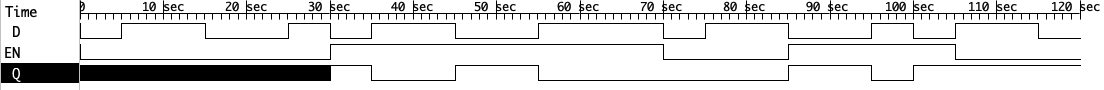
\includegraphics[scale=0.37]{img/gated_d1.png}
      \caption{Gated D latch simulation.} 
    \end{figure}
  \end{example} 

  This behavior is quite stable for storing 1-bit, but we need more control when storing a multi-bit buffer, where we need several D-latches working in tandem. The general idea is that if we have a multi-bit buffer, we want a set of D-latches to be enabled and disabled at once. So we could want something like this. 

  \begin{figure}[H]
    \centering 
    \begin{tikzpicture}
      \foreach \h in {0, 2, 4} {
        \draw (0, 0+\h) rectangle (0.8, 1.2+\h);
        \draw (-3, 1+\h) -- (0, 1+\h); 
        \draw (0.8, 0.65+\h) -- (2, 0.65+\h); 
        \node[right, font=\footnotesize] at (0, 1+\h) {$D$};
        \node[left, font=\footnotesize] at (0.8, 0.65+\h) {$Q$};
        \node[right, font=\footnotesize] at (0, 0.3+\h) {$E$};
        \draw (-1, 0.3+\h) -- (0, 0.3+\h);
        \fill (-1, 0.3+\h) circle (1.5pt);
      }
      \node[draw, circle] (clock) at (-4, -1) {clock};
      \draw (clock.east) -- (-1, -1) -- (-1, 4.3);
    \end{tikzpicture}
    \caption{Multiple D-latches enabled and disabled by some external source. The system clock would be a good candidate.} 
  \end{figure}

  \begin{figure}[H]
    \centering
    \begin{subfigure}[b]{0.32\textwidth}
      \centering
      \begin{tikzpicture}[circuit logic US]
        \node[and gate, scale=1.5] (and) at (3, 0) {};
        \node[not gate] (not) at (1, -0.3) {};
        \draw[blue] (-1, 0.2) -- (0, 0.2) -- (0, -0.3) -- (not.input);
        \draw[red] (not.output) -- (and.input 2); 
        \draw[blue] (-1, 0.2) -- (and.input 1); 
        \draw[blue] (and.output) -- (4, 0);
        \fill[blue] (0, 0.2) circle (1.5pt);
      \end{tikzpicture}
      \caption{By default the input current is $0$, and so the top input of the AND gate is $0$ and the bottom is $1$. }
    \end{subfigure}
    \hfill 
    \begin{subfigure}[b]{0.32\textwidth}
      \centering
      \begin{tikzpicture}[circuit logic US]
        \node[and gate, scale=1.5] (and) at (3, 0) {};
        \node[not gate] (not) at (1, -0.3) {};
        \draw[red] (-1, 0.2) -- (0, 0.2) -- (0, -0.3) -- (not.input);
        \draw[red] (not.output) -- (and.input 2); 
        \draw[red] (-1, 0.2) -- (and.input 1); 
        \draw[red] (and.output) -- (4, 0);
        \fill[red] (0, 0.2) circle (1.5pt);
      \end{tikzpicture}
      \caption{If the electric current of $1$ travels through the input wire, the top AND input becomes $1$. There is a small delay where the current does not reach the output of the NOT gate, so the output is $1$. }
    \end{subfigure}
    \hfill 
    \begin{subfigure}[b]{0.32\textwidth}
      \centering
      \begin{tikzpicture}[circuit logic US]
        \node[and gate, scale=1.5] (and) at (3, 0) {};
        \node[not gate] (not) at (1, -0.3) {};
        \draw[red] (-1, 0.2) -- (0, 0.2) -- (0, -0.3) -- (not.input);
        \draw[blue] (not.output) -- (and.input 2); 
        \draw[red] (-1, 0.2) -- (and.input 1); 
        \draw[blue] (and.output) -- (4, 0);
        \fill[red] (0, 0.2) circle (1.5pt);
      \end{tikzpicture}
      \caption{The signal goes through the NOT gate, turning the AND output back to $0$.}
    \end{subfigure}
    \caption{Blue means $0$, Red means $1$.}
  \end{figure}

  A clocked D latch is a D latch that is controlled by a clock signal. 

  \begin{definition}[Clocked D Latch]
    
  \end{definition}

  The most elementary chip is called a \textit{flip-flop}, of which there are many variants. In here, we will work with the data flip-flop. 

  \begin{definition}[Flip-Flop]
    A \textbf{data flip-flop (DFF)} is a device whose interface consists of a single-bit data input and single-bit data output. It also has a clock input that continuously changes accordingly to the master clock's signal. Taken together, the data and the clock inputs enable to the DFF to implement the time-based behavior 
    \begin{equation}
      \mathrm{out}(t) = \mathrm{in}(t - 1) 
    \end{equation}
    That is, the DFF outputs the input value from the previous time unit. 
  \end{definition}

  \begin{definition}[Register]
    
  \end{definition}

  \begin{definition}[Counter]
    
  \end{definition}

\subsection{Registers}

  To understand anything that the CPU does, we must understand assembly language. In here, everything is done within registers, and we can see how the CPU fetches, decodes, and executes instructions. So what exactly are these registers? 

  \begin{definition}[Register]
    A register is a small, fast storage location within the CPU. It is used to store data that is being used immediately, and is the only place where the CPU can perform operations, which is why it must move data from memory to registers before it can perform operations on it. Everything in a register is in binary, at most 8 bytes, or 64 bits. 

    There are very specific types of registers that you should know. All of these registers are implemented for all assembly languages and are integral to the workflow of the CPU.  
    \begin{enumerate}
      \item \textbf{parameter registers} which store the parameters of a function.
      \item \textbf{Return registers} which store return values of functions. 
      \item \textbf{stack pointers} which point to the top of the stack (at the top of the current stack frame). 
      \item \textbf{frame pointers} which point to the base of the current stack frame.
      \item \textbf{instruction pointers} which point to the next instruction to be executed.
    \end{enumerate}
  \end{definition}

  \begin{definition}[32 and 64 Bit Machines]
    There are two types of machines that tend to format these boxes very differently: 32-bit and 64-bit machines. 
    \begin{enumerate}
      \item 32 bit machines store addresses in 32 bits, so they can have $2^{32}$ addresses, which is about 4 GB of memory. 
      \item 64 bit machines store addresses in 64 bits, so they can have $2^{64}$ addresses, which is about 16 EB of memory. This does not mean that the actual RAM is 16 EB, but it means that the machine can \textit{handle} that much memory. 
      \begin{lstlisting} 
        ...
        0x00007FFF7FBFF860 --> 0b000000000000000000000000011111111111
                               111101111111101111111111100001100000
        0x00007FFF7FBFF861 --> 0b000000000000000000000000011111111111
                               111101111111101111111111100001100001
        0x00007FFF7FBFF862 --> 0b000000000000000000000000011111111111
                               111101111111101111111111100001100010
        0x00007FFF7FBFF863 --> 0b000000000000000000000000011111111111
                               111101111111101111111111100001100011
        0x00007FFF7FBFF864 --> 0b000000000000000000000000011111111111
                               111101111111101111111111100001100100
        ...
      \end{lstlisting}
    \end{enumerate}
    The numbers typically mean the size of the type that the machine works best with, so all memory addresses will be 32 or 64 bits wide. Most machines are 64-bits, and so everything in this notes will assume that we are working with a 64 bit machine. As we will later see, this is why pointers are 8 bytes long, i.e. 64 bits. This is because the memory addresses are 64 bits long, though all of them are not used. 
  \end{definition}

\subsection{Memory Banks}

  \begin{definition}[Memory]
    The \textbf{memory} is where the computer stores data and instructions, which can be though of as a giant array of memory addresses, with each containing a byte. This data consists of graphical things or even instructions to manipulate other data. It can be visualized  as a long array of boxes that each have an \textbf{address} (where it is located) and \textbf{contents} (what is stored in it).

    Memory simply works as a bunch of bits in your computer with each bit having some memory address, which is also a bit. For example, the memory address \texttt{0b0010} (2) may have the bit value of \texttt{0b1} (1) stored in it. 

    \begin{figure}[H]
      \centering 
      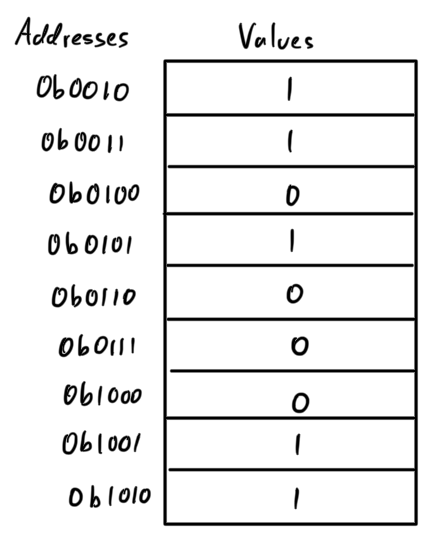
\includegraphics[scale=0.4]{img/memory_visual_bit.png}
      \caption{Visualization of memory as a long array of boxes of bits. }
      \label{fig:memory_visual_bit}
    \end{figure}

    However, computers do not need this fine grained level of control on the memory, and they really work at the Byte level rather than the bit level. Therefore, we can visualize the memory as a long array of boxes indexed by \textit{Bytes}, with each value being a byte as well. In short, the memory is \textbf{byte-addressable}. In certain arthitectures, some systems are \textbf{word-addressable}, meaning that the memory is addressed by words, which are 4 bytes.\footnote{Note that in here the size of a word is 2 bytes rather than 4 as stated above. This is just how it is defined in some \texttt{x86} architectures.}

    \begin{figure}[H]
      \centering 
      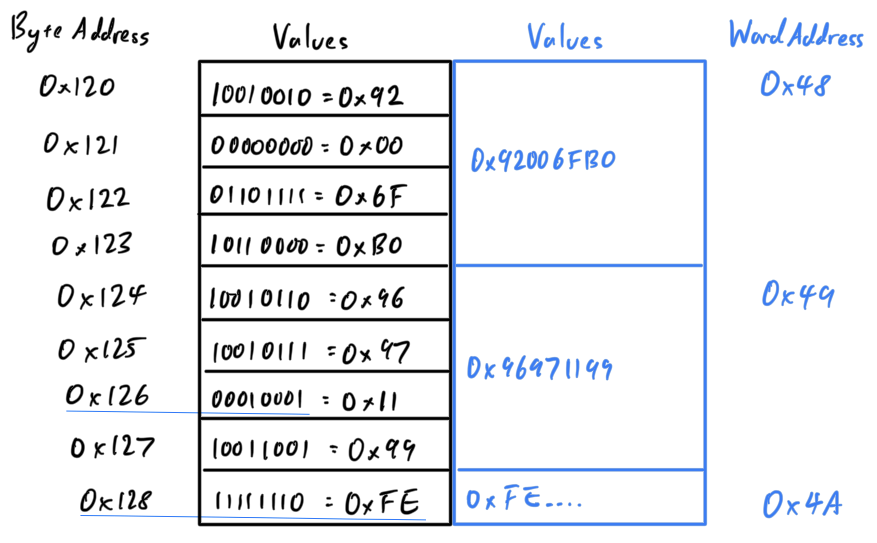
\includegraphics[scale=0.4]{img/memory_visual_byte.png}
      \caption{Visualization of memory as a long array of boxes of bytes. Every address is a byte and its corresponding value at that address is also a byte, though we represent it as a 2-digit hex. } 
      \label{fig:memory_visual_byte}
    \end{figure}
  \end{definition}

  It is intuitive to think that given some multi-byte object like an \texttt{int} (4 bytes), the beginning of the int would be the lowest address and the end of the int would be the highest address, like how consecutive integers are stored in an array. However, this is not always the case (almost always not the case since most computers are little-endian).  

  \begin{definition}[Endian Architecture]
    Depending on the machine architecture, computers may store these types slightly differently in their \textit{byte} order. Say that we have an integer of value \texttt{0xA1B2C3D4} (4 bytes). Then, 
    \begin{enumerate} 
      \item A \textbf{big-endian architecture} (e.g. SPARC, z/Architecture) will store it so that the least significant byte has the highest address.
      \item A \textbf{little-endian architecture} (e.g. x86, x86-64, RISC-V) will store it so that the least significant byte has the lowest address. 
      \item A \textbf{bi-endian architecture} (e.g. ARM, PowerPC) can specify the endianness as big or little. 
    \end{enumerate}

    \begin{figure}[H]
      \centering 
      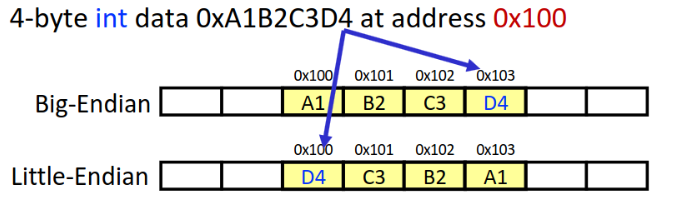
\includegraphics[scale=0.4]{img/endianness.png}
      \caption{The big vs little endian architectures. } 
      \label{fig:endianness}
    \end{figure}
  \end{definition}

  We can simply print out the hex values of primitive types to see how they are stored in memory, but it does not provide the level of details that we want on which bytes are stored where. At this point, we must use certain \textbf{debuggers} to directly look at the memory. For x86 architectures, we can use \texttt{gdb} and for ARM architectures, we can use \texttt{lldb}. At this point, we need to understand assembly to look through debuggers, so we will provide the example here. 

  \begin{example}[Endianness of C Int in x86-64]
    To do. 
  \end{example}

  \begin{example}[Endianness of C Int in ARM64]
    To do. 
  \end{example}

\subsection{Counter Chips}

\subsection{Memory Management Unit}

